\documentclass[tikz,border=8pt]{standalone}
% Shared look for every TikZ diagram. Load with \input{../../tools/tikz-style.tex}
\usepackage[T1]{fontenc}
\usepackage{lmodern}
\renewcommand{\sfdefault}{lmr}  % diagrams use the same serif as the text
\usetikzlibrary{arrows.meta, positioning, shapes.geometric, calc, fit, backgrounds}
\definecolor{cblue}{HTML}{4C78A8}
\definecolor{corange}{HTML}{F58518}
\definecolor{cgreen}{HTML}{54A24B}
\definecolor{cred}{HTML}{E45756}
\definecolor{cpurple}{HTML}{B279A2}
\definecolor{cgrey}{HTML}{6B6B6B}
\tikzset{
  every picture/.style={font=\sffamily, line width=1.2pt},
  box/.style={draw=#1, fill=#1!12, rounded corners=4pt, align=center, inner sep=7pt, minimum height=1.1cm},
  box/.default=cgrey,
  arrow/.style={-{Stealth[length=3mm]}, draw=cgrey, line width=1.4pt},
  title/.style={font=\sffamily\bfseries\Large},
  note/.style={font=\sffamily\small, text=cgrey, align=center},
}
\AtBeginDocument{\hyphenpenalty=10000 \exhyphenpenalty=10000}

\begin{document}
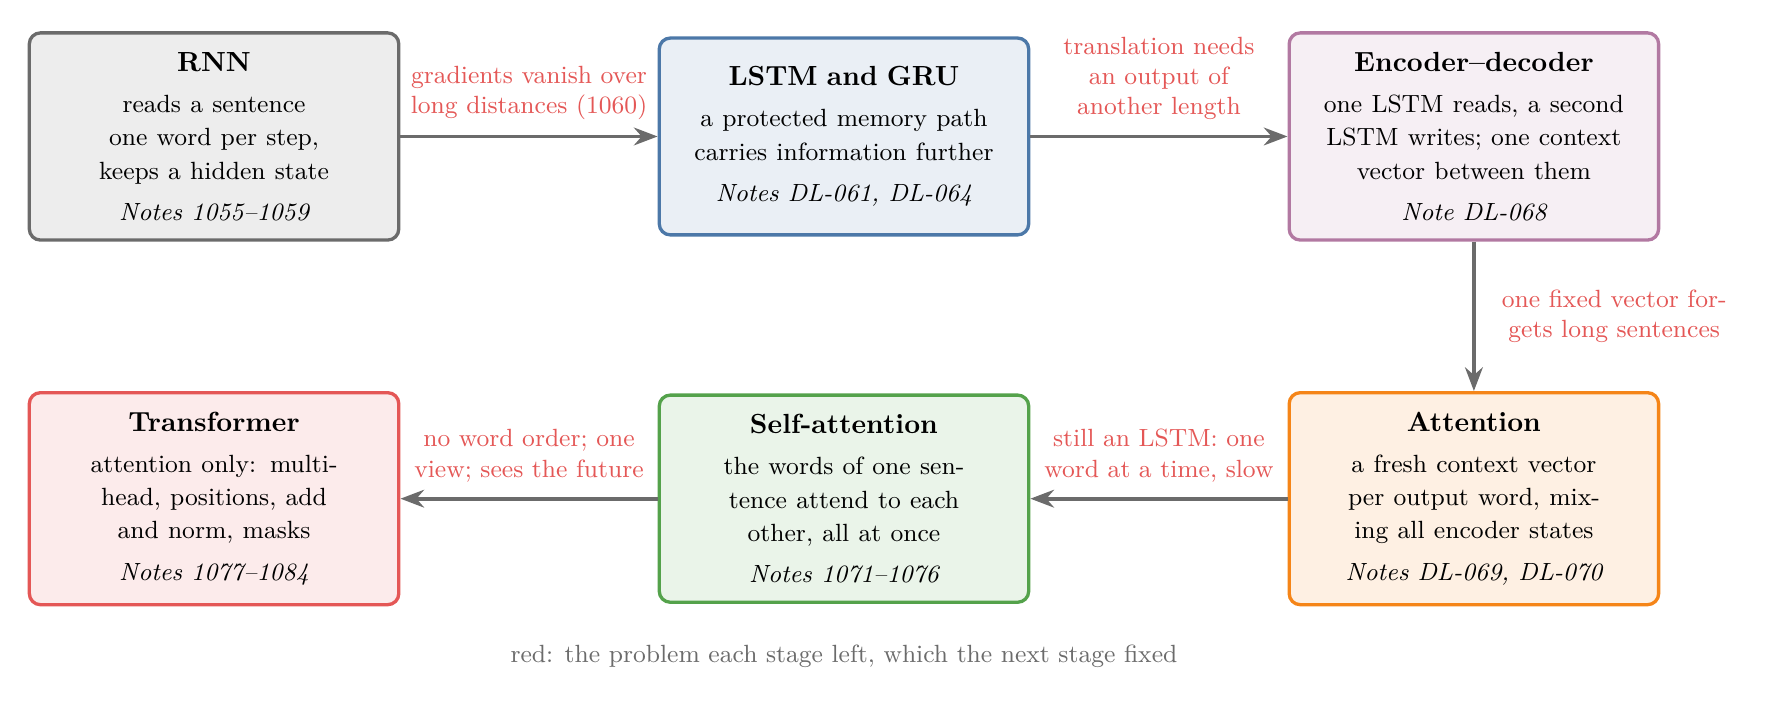
\begin{tikzpicture}[stage/.style={box=#1, text width=4.2cm, minimum height=2.5cm, font=\sffamily},
  prob/.style={font=\sffamily\small, text=cred, align=center, text width=3.1cm}]
  \foreach \i/\c/\x/\y/\name/\idea/\notes in {
    1/cgrey/0/0/{RNN}/{reads a sentence one word per step, keeps a hidden state}/{Notes 1055--1059},
    2/cblue/8/0/{LSTM and GRU}/{a protected memory path carries information further}/{Notes DL-061, DL-064},
    3/cpurple/16/0/{Encoder--decoder}/{one LSTM reads, a second LSTM writes; one context vector between them}/{Note DL-068},
    4/corange/16/-4.6/{Attention}/{a fresh context vector per output word, mixing all encoder states}/{Notes DL-069, DL-070},
    5/cgreen/8/-4.6/{Self-attention}/{the words of one sentence attend to each other, all at once}/{Notes 1071--1076},
    6/cred/0/-4.6/{Transformer}/{attention only: multi-head, positions, add and norm, masks}/{Notes 1077--1084}} {
    \node[stage=\c] (s\i) at (\x, \y) {\textbf{\name}\\[3pt]{\small \idea}\\[3pt]{\small\itshape \notes}};
  }
  \draw[arrow] (s1.east) -- node[prob, above=2pt] {gradients vanish over long distances (1060)} (s2.west);
  \draw[arrow] (s2.east) -- node[prob, above=2pt] {translation needs an output of another length} (s3.west);
  \draw[arrow] (s3.south) -- node[prob, right=4pt, text width=3.0cm] {one fixed vector forgets long sentences} (s4.north);
  \draw[arrow] (s4.west) -- node[prob, above=2pt] {still an LSTM: one word at a time, slow} (s5.west -| s5.east);
  \draw[arrow] (s5.west) -- node[prob, above=2pt] {no word order; one view; sees the future} (s6.east);
  \node[note] at (8, -6.6) {red: the problem each stage left, which the next stage fixed};
\end{tikzpicture}
\end{document}
